\documentclass{beamer}
\usetheme{metropolis}

\usepackage{enumitem}
\setlist[itemize,1]{before*=\normalsize,label=$\bullet$}
\setlist[itemize,2]{before*=\small,label=$\circ$}
\setlist[itemize,3]{before*=\footnotesize,label=\Smiley}

\usepackage{marvosym}
\usepackage{tikz}

\title{%
  Discrete Channels w/Noise \\
  \normalsize A Mathematical Theory of Communication, Part II}
\author{David Sanders}

\begin{document}

  \maketitle

  \section{First, some review... \\
           \small (p.1 -- 19 of Shannon)}

  \begin{frame}{Introduction}
    \begin{itemize}
      \item Context of signal processing (PCM, PPM)
      \item Communication is reproducing messages sent over channels
      \item Mathematical theory shouldn't care about meaning
      \begin{itemize}
        \item Instead, focus on message as one selected from many possibilities
        \item Absence of meaning allows message to be viewed as random variable
      \end{itemize}
      \item Any monotonic, increasing function of number of possibilities $n$
      is measure of information
      \begin{itemize}
        \item Use $\log n$
        \begin{itemize}
          \item Engineering parameters vary linearly w/log of possibilities
          \item More intuitive -- 2 disks have twice the information ($(2^x)(2^x) = 2^{2x}$ states)
          \item Mathematically convenient -- ``downgrades" operations; $\log ab
          = \log a + \log b$, $\log x^a = a \log x$, etc.
        \end{itemize}
      \end{itemize}
    \end{itemize}
  \end{frame}

  \section{Discrete Noisy Channels \\
           \small (p.19 -- 28 of Shannon)}

  \begin{frame}{Basic Concepts \small (p.19)}
    What is noise ($N$)?
    \begin{itemize}
      \item Perturbation of transmitted signal ($S$) at either terminal or in
      channel
      \item Received signal ($E$) may not be same as transmitted signal ($S$)
    \end{itemize}

    \begin{figure}
      \footnotesize
      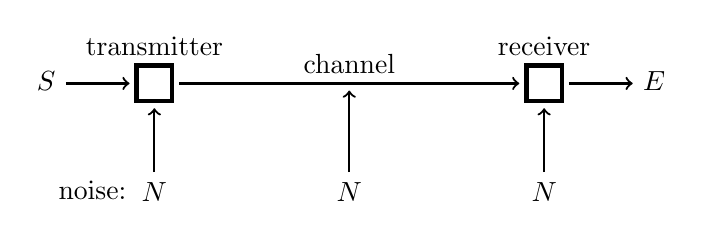
\begin{tikzpicture}[scale=0.45,->,thick]
        \draw (-2,0.5) -- (-0.2,0.5);
        \node [left] at (-2,0.575) {$S$};
        \node [below left] at (0,-1.95) {noise:};

        \draw (0.5,-2) -- (0.5,-0.2);
        \node [below] at (0.5,-2) {$N$};

        \draw [ultra thick] (0,0) rectangle (1,1);
        \node [above] at (0.5,1) {transmitter};

        \draw (1.2,0.5) -- (10.8,0.5);
        \node [above] at (6,0.5) {channel};

        \draw (6,-2) -- (6,0.3);
        \node [below] at (6,-2) {$N$};

        \draw [ultra thick] (11,0) rectangle (12,1);
        \node [above] at (11.5,1) {receiver};

        \draw (11.5,-2) -- (11.5,-0.2);
        \node [below] at (11.5,-2) {$N$};

        \draw (12.2,0.5) -- (14,0.5);
        \node [right] at (14,0.575) {$E$};
      \end{tikzpicture}
      \caption{Sources of noise.}
    \end{figure}
  \end{frame}

  \begin{frame}{Kinds of Noise \small (p.19)}
    Two different kinds of noise:
    \begin{itemize}
      \item Distortion: $E \neq S$ and $E = f(S)$
      \begin{itemize}
        \item If $f^{-1}$ exists for $f$, recovery of $S$ from $E$ is possible
      \end{itemize}
      \item Random noise: $E \neq S$ and $E = f(S, N)$
      \begin{itemize}
        \item Noise $N$ is random variable; may be represented by stochastic
        process
      \end{itemize}
    \end{itemize}
  \end{frame}

  \begin{frame}{Generalization \small (p.19)}
    Generalization via finite-state, noise-free channel:
    \begin{equation}
    p_{\alpha,i}(\beta,j)
    \end{equation}
    Probability, if channel in state $\alpha$ and symbol $i$ transmitted, that
    symbol $j$ received and channel left in state $\beta$.

    If symbols independently perturbed by noise, channel state omitted (only
    one state):
    \begin{equation}
    p_{i}(j)
    \end{equation}
    Probability, if symbol $i$ transmitted, that symbol $j$ received.
  \end{frame}

  \begin{frame}{Different Entropies \small (p.19)}
    In noisy channel, two statistical processes:
    \begin{itemize}
      \item Source
      \item Noise
    \end{itemize}
    Therefore, a number of different entropies are considered:
    \begin{itemize}
      {\small
        \item $H(x)$ -- entropy of transmitted signal
        \item $H(y)$ -- entropy of received signal
        \item $H(x,y)$ -- joint entropy of transmitted and received signals
        \item $H_x(y)$ -- entropy of received signal when transmitted signal is known
        \item $H_y(x)$ -- entropy of transmitted signal when received signal is known
      }
    \end{itemize}
  \end{frame}

  \begin{frame}{Relationship of Entropies \small (p.19)}
    Relationship of previous entropies given below:
    \begin{equation}
      H(x,y) = H(x) + H_x(y) = H(y) + H_y(x)
    \end{equation}
    More descriptively,
    \begin{itemize}
      \item $H(x,y) = H(x) + H_x(y)$ -- joint entropy is entropy of $x$ plus
      entropy of $y$ not accounted for by $x$
      \item $H(x,y) = H(y) + H_y(x)$ -- joint entropy is entropy of $y$ plus
      entropy of $x$ not accounted for by $y$
    \end{itemize}
    With no noise,
    \begin{itemize}
      \item $H(x,y) = H(x)$ and $H_x(y) = 0$
      \item Or, $H(x,y) = H(y)$ and $H_y(x) = 0$
    \end{itemize}
  \end{frame}

  \begin{frame}{An Example \small (p.20)}
    An example,
    \begin{itemize}
      \item Symbols $0$ and $1$
      \item Probabilities $p_0 = p_1 = \frac{1}{2}$
      \item $1000$ symbols per second
      \item $\implies$ $1000$ bits per second
    \end{itemize}
    If noise causes $1$ in $100$ symbols ($1\%$) to be received incorrectly,
    what is overall rate of transmission?
    \begin{itemize}
      \item Definitely $< 1000$ bits per second
      \item $1000 \times 0.01 = 990$ bits per second?
    \end{itemize}
  \end{frame}

  \begin{frame}{An Example \small (p.20)}
    If rate of transmission is $1000 \times 0.01 = 990$ bits per second, then
    error rate of $50\%$ would still permit transmission of $500$ bits per
    second even though message is completely unintelligible.  So this is
    clearly not the answer.  Then what is?
  \end{frame}

  \begin{frame}{An Example \small (p.20)}
    Must subtract from transmitted information $H(x)$ the portion of $H(x)$
    missing in received information $H(y)$.  Alternatively, the uncertainty in
    the transmitted information $H(x)$ given that we know the received signal
    $y$:
    \begin{equation}
      R = H(x) - H_y(x)
    \end{equation}
    $R$ is the actual rate of transmission.  $H_y(x)$ is the
    \emph{equivocation} (average ambiguity of received signal).
  \end{frame}

  \begin{frame}{An Example \small (p.20)}
    Given received signal, two possible outcomes regarding transmitted signal:
    \begin{itemize}
      \item Correct symbol was received with probability $p_{correct}$
      \item Incorrect symbol was received with probability $p_{incorrect}$
    \end{itemize}
  \end{frame}

  \begin{frame}{An Example \small (p.20)}
    In previous example,
    \begin{itemize}
      \item $p_{correct} = 0.99$ and $p_{incorrect} = 0.01$
      \item $H_y(x) = -\left[ 0.99 \log 0.99 + 0.01 \log 0.01 \right] \approx 0.081$ bits per symbol
      \item $R \approx 1000 - 81 = 919$ bits per second
    \end{itemize}
    If $p_{correct} = p_{incorrect} = \frac{1}{2}$,
    \begin{itemize}
      \item $H_y(x) = -\left[ 0.5 \log 0.5 + 0.5 \log 0.5 \right] = 1$ bits per symbol
      \item $R = 1000 - 1000 = 0$ bits per second
    \end{itemize}
  \end{frame}

\end{document}
